\section{Model problema}
\label{sec:model_problema}

Projekt optimizacije raspodjele projektnih aktivnosti može se formalno predstaviti kao skup od $n$ zadataka, pri čemu svaki zadatak $i$ ima definirane sljedeće karakteristike:
\begin{itemize}
    \item \textbf{procijenjeno trajanje} $d_i$,
    \item \textbf{trošak} $c_i$,
    \item \textbf{vrijednost} odnosno povrat ulaganja (ROI) $v_i$,
    \item \textbf{distribucija nesigurnosti} koja opisuje varijabilnost trajanja i/ili troška.
\end{itemize}

Ovakav formalizam omogućuje primjenu metoda kombinatorne optimizacije \cite{Glover1986} i stohastičkih simulacija \cite{Law2015} za donošenje optimalnih odluka u uvjetima ograničenih resursa.

\subsection{Ograničenja}
Projekt je podložan realnim ograničenjima resursa, koja se u modelu izražavaju na sljedeći način:
\begin{align}
    \sum_{i=1}^n d_i &\leq T_{\mathrm{max}} \quad \text{(ukupno vrijeme)} \label{eq:time_constraint} \\
    \sum_{i=1}^n c_i &\leq B_{\mathrm{max}} \quad \text{(budžet)} \label{eq:budget_constraint} \\
    \sum_{i=1}^n r_i &\leq R_{\mathrm{max}} \quad \text{(maksimalan broj radnika)} \label{eq:workers_constraint}
\end{align}
gdje $T_{\mathrm{max}}$ označava raspoloživo ukupno vrijeme, $B_{\mathrm{max}}$ raspoloživi budžet, a $R_{\mathrm{max}}$ maksimalan broj raspoloživih radnika.

\subsection{Cilj optimizacije}
Cilj optimizacije je \textbf{maksimizirati ukupnu vrijednost projekta} ostajući unutar svih definiranih ograničenja:
\begin{equation}
    \max \sum_{i=1}^n v_i \cdot x_i
    \label{eq:objective}
\end{equation}
pri čemu $x_i \in \{0,1\}$ označava binarnu varijablu koja označava odabir zadatka $i$ za izvršenje.

\subsection{Grafički prikaz modela}
Na slici \ref{fig:model_problema} prikazan je konceptualni model problema optimizacije raspodjele projektnih aktivnosti, uključujući ulazne podatke, ograničenja i ciljnu funkciju.

\begin{figure}
    \centering
    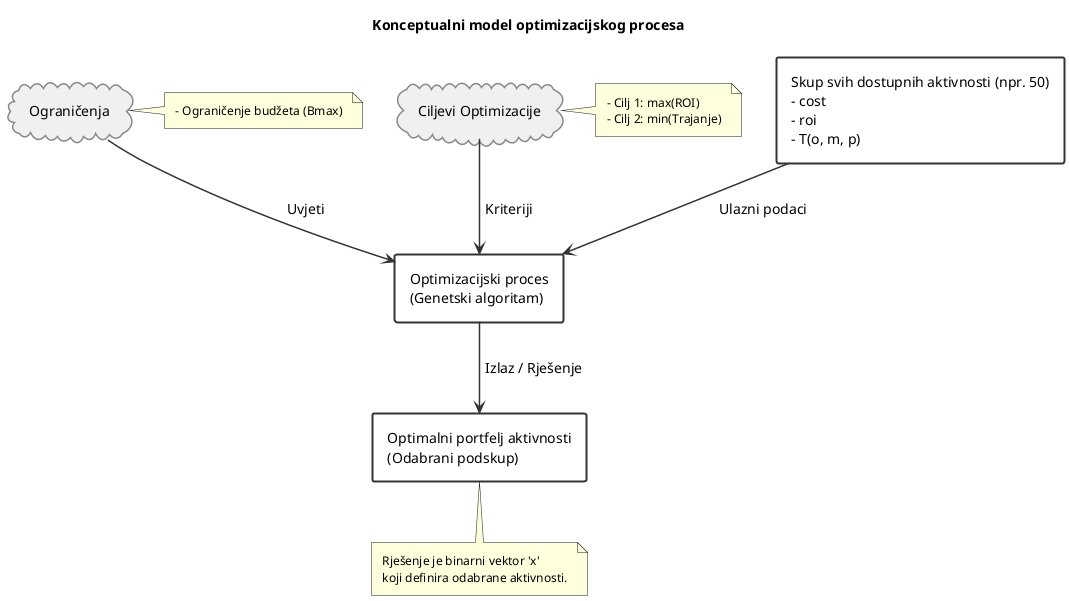
\includegraphics[width=0.9\textwidth]{slike/model_problema.png}
    \caption{Model problema optimizacije raspodjele projektnih aktivnosti}
    \label{fig:model_problema}
\end{figure}

\subsection{Zaključak poglavlja}
Ovaj model problema omogućuje matematičku i vizualnu formalizaciju optimizacijskog zadatka. Jasna definicija ulaza, ograničenja i cilja ključna je za primjenu optimizacijskih metoda poput genetskih algoritama \cite{Goldberg1989} u kombinaciji s Monte Carlo simulacijama kako bi se dobila rješenja visoke kvalitete u uvjetima nesigurnosti.
